%compile with XeLaTeX, biber, xelatex, xelatex
\documentclass[11pt,a4paper,titlepage]{article}
\usepackage[utf8]{inputenc}
\usepackage[main=german,english]{babel}
\usepackage[T1]{fontenc}
\usepackage{fontspec}
\setmainfont{Arial}
\usepackage{amsmath}
\usepackage{amsfonts}
\usepackage{amssymb}
\usepackage{graphicx}
\usepackage[onehalfspacing]{setspace}
\usepackage[left=2cm,right=2cm,top=2cm,bottom=2cm]{geometry}
\graphicspath{{./img/}}
\usepackage{titlepic}
\usepackage[document]{ragged2e}
\usepackage{float}
\usepackage[titles]{tocloft}
\usepackage[style=ieee,backend=biber,alldates=iso]{biblatex}
\addbibresource{darwin-fachartikel.bib}

	
\titlepic{
\includegraphics[width=\textwidth]{darwin.png}}

\author{
Michael Schaufelberger (Product Owner)\\
Filip Kašiković (Scrum Master)\\
Raphael Mailänder\\
Simon Stucki\\
Marc Berli\\
Ferenc Kuntič}

%%% TODO: HINWEIS AUF ZHAW SCHÖNER FORMATIEREN
\title{{\small ZHAW School of Engineering, 
IT17ta\_ZH, 
PSIT 4}\\
Projekt Darwin}

\begin{document}

\maketitle

%%% TODO: englisch machen geht nicht solange sprache deutsch eingestellt ist...
\begin{otherlanguage}{english}
\begin{abstract}

%250 wörter
% Einleitung: Definiere Problematik und begründe Revelanz der Untersuchung
In der heutigen Zeit haben sich Videospiele in unserer Gesellschaft stark etabliert und sind ein Teil unseres Alltags geworden. Die Branche und Präsenz der Spieleindustrie wächst von Jahr zu Jahr stetig an und bildet ein sehr lukratives Geschäftsumfeld. Erträge und Umsätze in Milliardenhöhe sind keine Seltenheit. Unternehmen mit mehreren hundert Mitarbeitern, versuchen im Schnelltempo Spiele verschiedenster Art auf den Markt zu bringen. 

Angesichts solch grosser Konkurrenz stellen sich uns die Fragen: Wie gestalten wir ein attraktives Spiel? Wer ist die Zielgruppe? Wie können wir die Spieler für das Spiel begeistern? Welche Qualitäten braucht das Spiel?
\\Um all diese Fragen beantworten zu können, braucht es ein fundiertes Konzept, durchdachte Überlegungen und ein gutes Team. Obwohl die Konkurrenz sehr gross ist, sehen wir eine Möglichkeit, mit einem interaktiven Mehrspieler-Spiel den Durchbruch zu schaffen.

% Methodische Einordnung: Art und Ziel der Arbeit (Umfrage, Analyse, Test, etc)
Ziel dieser Arbeit ist es, ein innovatives und erfinderisches Spiel zu entwickeln, das sowohl logisches Denken wie auch technisches Interesse fördert. Das Ziel des Spieles ist es, Spieleinheiten mit kleinen Code-Abschnitten zu steuern und schlussendlich der letzte ''Überlebende'' zu sein.

% Vorgehen:  Typische Fragestellungen werden genannt oder ein Testbeispiel wird beschrieben
Bei der Entwicklung werden modernste Technologien eingesetzt. Für den Frontend-Bereich haben wir uns für React entscheiden. Dies ermöglicht es uns die Applikation in Komponenten zu entwickeln und erhöht den Wiederverwendungsgrad. Für die Realisierung des Backends setzen wir auf Node.js und TypeScript, da es uns erlaubt die Applikation modularer zu bauen und sie eine grosse Community besitzen.
Für das Projektmanagement der Entwicklung wurde uns Scrum als agilen Prozess vorgegeben.

% Ergebnis: Beschreibt wichtigste Resultalte, Erkenntnisse, offene Fragen
Das Ergebnis des ''Projekt Darwin'' ist ein herausforderndes Überlebensspiel, in dem mehrere Spieler gegeneinander antreten können.

\end{abstract}
\end{otherlanguage}

%\tableofcontents

\newpage

\pagestyle{myheadings}
\markright{\hfill Projekt Darwin \hfill}

\section{Einleitung}

% bestehende arbeiten/Literatur
% stand der technik / bisherige Lösungen des Problems, deren Grenzen

Bestehende Spiele, die mittels Programmierung gesteuert werden, zielen sehr stark darauf ab die Programmierfähigkeiten zu verbessern, oder ganz grundlegend, die beim Programmieren notwendige Art des Denkens zu vermitteln.
Die meisten dieser Spiele sind für Kinder gemacht, da diese möglichst spielerisch dazu gebracht werden wollen, Dinge zu erlernen. Allerdings wissen auch grössere Kinder eine spielerische Lernweise zu schätzen.

Bei vielen der Lösungen steht das Programmieren im Vordergrund - die Grafik und damit auch der Spielspass, lassen zu wünschen übrig.
Weiter sind die meisten der Konkurrenzprodukte nur für einen Spieler ausgelegt (''Single Player''). Auch dies limitiert den Spielspass.
Um diese Schwächen zu adressieren, haben wir ''Projekt Darwin'' entwickelt.

\subsection{Zielsetzungen}

% ziel der arbeit
%verweis auf offizielle aufgabenstellung im anhang:
%% successfully develop a complex software system in a large team of 7+2 students
%% strengthen agile software engineering competences
% übersicht über die arbeit, stellt die folgenden teile kurz vor
% angaben zum zielpublikum, nennt das vorausgesetzte wissen
% terminologie, definition der verwendeten begriffe


Ziel von ''Projekt Darwin'' ist es, sowohl den Spielspass zu maximieren, als auch die algorithmische, logische Denkweise zu fördern. Das Spiel soll sowohl von Kindern als auch von Erwachsenen gespielt werden können, wobei die Grafik insbesondere nicht kindlich sein soll.
Das Spiel in seiner jetzigen Version lässt sich mit wenigen Befehlen spielen, weshalb nur minimale, technische Vorkenntnisse nötig sind.
In einer zukünftigen Version könnte man das verwendete Set an Befehlen in höheren Levels erweitern, sodass die Komplexität zunimmt und der Spieler im Laufe der Zeit dazulernen kann.
Ein weiteres Ziel des Projektes ist es, die Kompetenzen des Entwicklungsteams bezüglich agiler Software-Entwicklung aufzubauen und zu festigen.

\newpage

\section{Resultate}
% Zusammenfassung der Resultate. Beschreibung der Lösung z. B. gemäss Report?
In diesem Kapitel werden die Resultate und Ergebnisse dieses Projektes präsentiert.
Es wird auf die einzelnen Bausteine der Applikation detaillierter eingegangen und die Lösungsentscheide beschrieben, die innerhalb des Teams getroffen wurden.

%Jeweils ein code snippet als beispiel einbinden ?
\subsection{Technische Design-Entscheidungen}
Für die Umsetzung des Projekts waren verschiedene technische Entscheidungen nötig, die im Folgenden erläutert werden.
\subsubsection{TypeScript / Node.js}
TypeScript ist eine Programmiersprache, die von Microsoft entwickelt wurde und Code in JavaScript kompiliert. Durch die Typisierung ermöglicht sie es, verschiedene Module besser zu organisieren und Refactoring einfacher durchzuführen.
Da es sich bei Darwin um eine Webapplikation handelt, welche in Frontend und Backend aufgeteilt ist, und aufgrund der Erfahrung der Teammitglieder, ist die Entscheidung gefallen, ausschliesslich TypeScript einzusetzen.
Mithilfe von TypeScript kann der Quellcode mit einer besseren Struktur versehen werden (siehe zum Beispiel die Struktur der Spielobjekte in Abb. \ref{types}) und ihn besser formulieren sowie auch einfacher skalieren.

\begin{figure}[H]
	\centering
	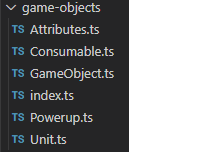
\includegraphics{darwintypes.png}
	\caption{Datei- und Ordnerstruktur der Spielobjekte}
	\label{types}
\end{figure}

Mittels Node.js kann sowohl im Frontend als auch im Backend JavaScript eingesetzt werden. Dies ermöglicht es uns, Code einfacher zwischen den verschiedenen Teilen der Applikation wiederzuverwenden. Zudem ist es eine sehr beliebte JavaScript Runtime \cite{node-git} und weist die notwendige Stabilität für das Projekt Darwin auf.

\subsubsection{React / 2D Canvas}
React ist eine JavaScript-Bibliothek, deren Ziel es ist, die Entwicklung von grafischen Benutzeroberflächen im Webbrowser zu vereinfachen. Sie wurde 2013 von Facebook entwickelt \cite{react-handbook} und ist in der Web-Entwicklung mittlerweile stark verbreitet.
Aufgrund der bestehenden Erfahrung des Teams und einer sehr grossen Community, fiel der Entscheid leicht, React zu benutzen.
Für die Visualisierung des Spiels und dessen Objekte wird ein 2D Canvas mittels Pixi.js eingesetzt. Der Einsatz von Pixi.js erlaubt es, die Canvas API zu abstrahieren und somit den Aufwand für die Umsetzung der Visualisierung zu verringern.

\subsubsection{Lerna / Monorepo}
Lerna ist ein Tool, das die Verwaltung von Repositories mit mehreren Paketen mittels Git und NPM, dem Paketmanager von Node.js, optimiert \cite{lerna}. Bei diesem Projekt hilft Lerna mit der Verwaltung von Paketen, die sowohl im Frontend als auch im Backend verwendet werden.

\subsubsection{Testing / Jest}
Unit Tests werden automatisch bei jedem Build ausgeführt.
Als Framework wird Jest von Facebook verwendet. Dieses ist in der JavaScript-Community weit verbreitet und im Team ist bereits Know-How vorhanden.
Beim Unit Testing werden einzelne Einheiten isoliert getestet und sowohl im Frontend als auch im Backend separat ausgeführt.

\subsubsection{Workflow / CI|CD}
Ein reibungsloser Entwicklungsprozess hat für das Entwicklungsteam oberste Priorität. Deswegen wurde beschlossen eine Build- sowie eine Releasepipeline einzurichten (siehe Abb. \ref{pipeline}). Diese ermöglicht es, Pull-Requests automatisch zu testen und bei einem erfolgten Merge automatisiert zu Deployen.

\begin{figure}[H]
	\centering
	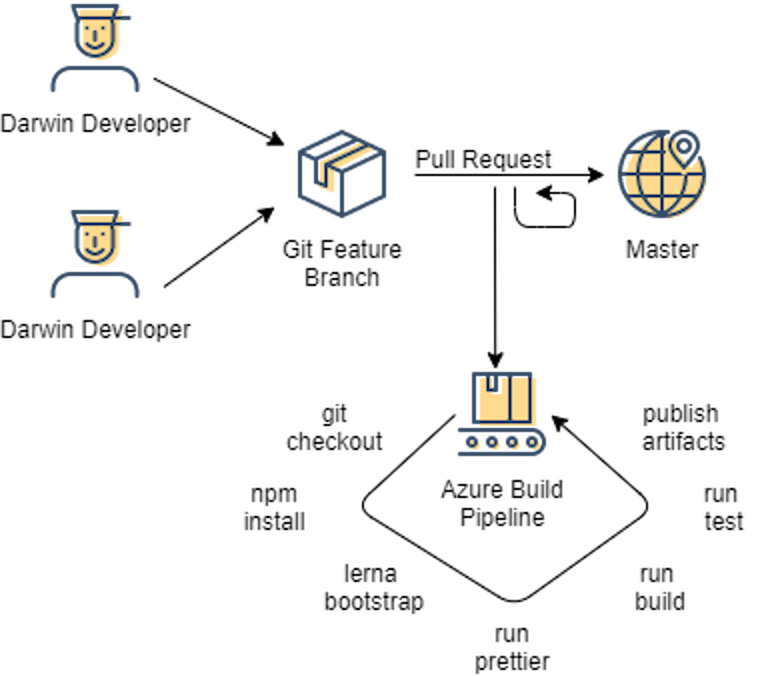
\includegraphics{workflow.png}
	\caption{Entwicklungsprozess und CI/CD-Pipeline}
	\label{pipeline}
\end{figure}

\pagebreak

\subsection{Implementiertes Spiel}

In diesem Abschnitt werden die Elemente des implementierten Spiels beschrieben.

\subsubsection{Benutzeroberfläche}

Wie in Abbildung \ref{gameplay} ersichtlich ist, gliedert sich die Benutzeroberfläche in ein Spielfeld (rechts) und ein Eingabefeld (links), durch das der Spieler den Spielverlauf steuern kann. Innerhalb des Spiels ist eine detaillierte Hilfeseite mit Beispielen direkt unter dem Spielfeld einsehbar.

\begin{figure}[H]
	\centering
	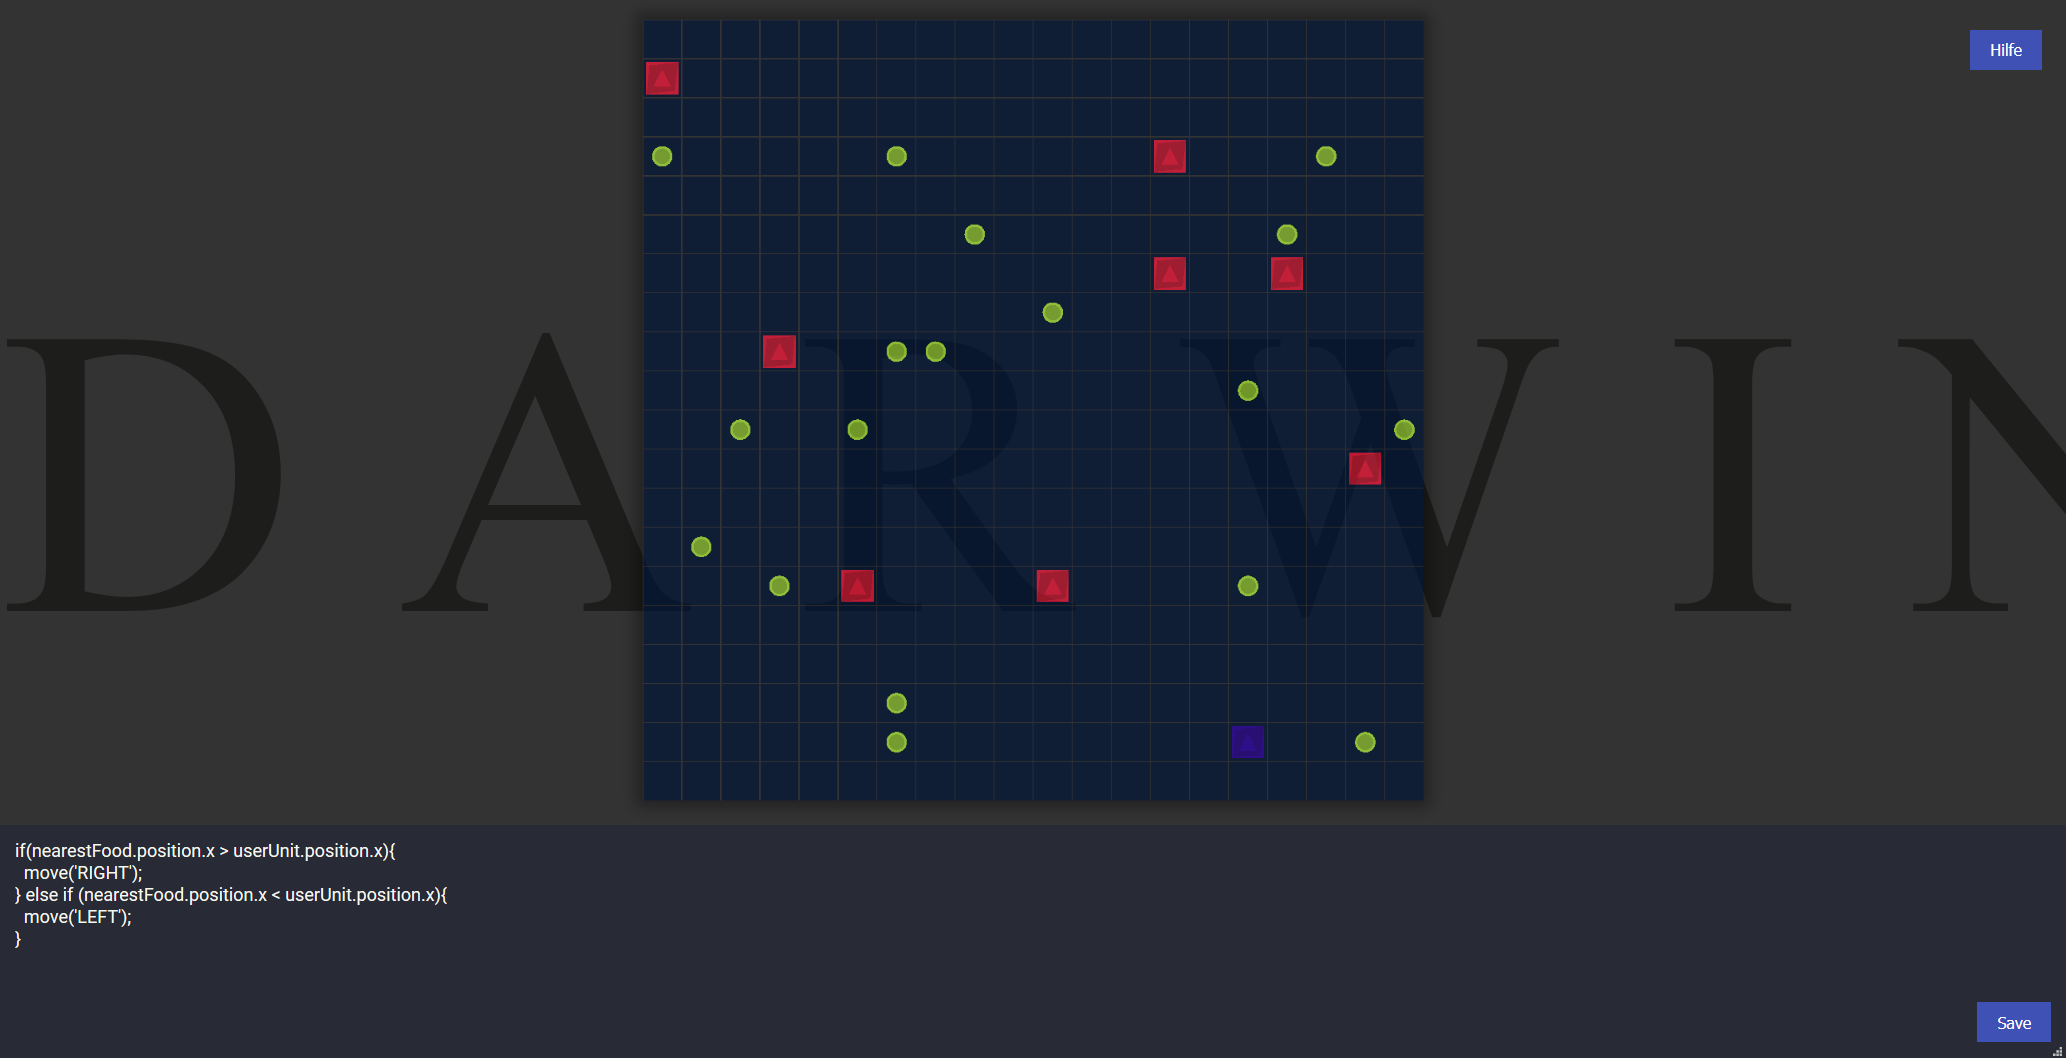
\includegraphics[width=\textwidth]{darwin-gameplay.png}
	\caption{Layout der Benutzeroberfläche}
	\label{gameplay}
\end{figure}

\subsubsection{Spielfeld}

Das Spielfeld (sichtbar in Abb. \ref{spielfeld}) ist in ein Raster unterteilt. Die Spielobjekte werden als geometrische Figuren visualisiert. Diese geometrischen Formen haben folgende Bedeutung:
\begin{itemize}
\item Grünes Quadrat: Der aktuelle Spieler (''ich'')
\item Rotes Quadrat: Anderer Spieler (''Gegner'')
\item Balken über den Quadraten: Gesundheitszustand des Spielers (''Health'')
\item Blauer Kreis: Nahrung
\item Kleine Quadrate (verschiedene Farben): ''Power-Ups'', die Spieler temporär beeinflussen, falls diese konsumiert werden.
\end{itemize}

\begin{figure}[H]
	\centering
	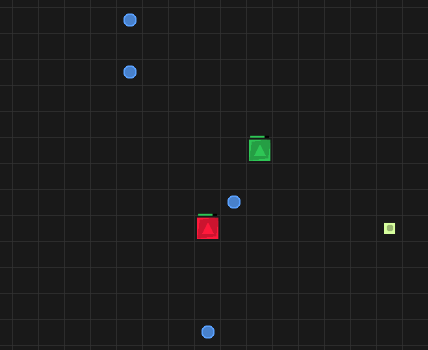
\includegraphics{game1.png}
	\caption{Design Spielfeld}
	\label{spielfeld}
\end{figure}

\subsubsection{Spielführung}

Gespielt wird mittels Code-Eingabe, zum Beispiel \texttt{move('LEFT')}, wie in Abbildung \ref{code-eingabe} ersichtlich. Ziel ist es, als Letzter zu überleben. Um am Leben zu bleiben, muss man Nahrung sammeln. Das Konsumieren von Powerups kann dem Spieler einen entscheidenden Vorteil verschaffen, um den Sieg zu erlangen. Ist man gerüstet, kann der Spieler auch gegnerische Spieler angreifen, um dem Sieg ein Stück näher zu kommen. Aber hierbei ist Vorsicht geboten: Dieses Manöver kann nach hinten los gehen!

\begin{figure}[H]
	\centering
	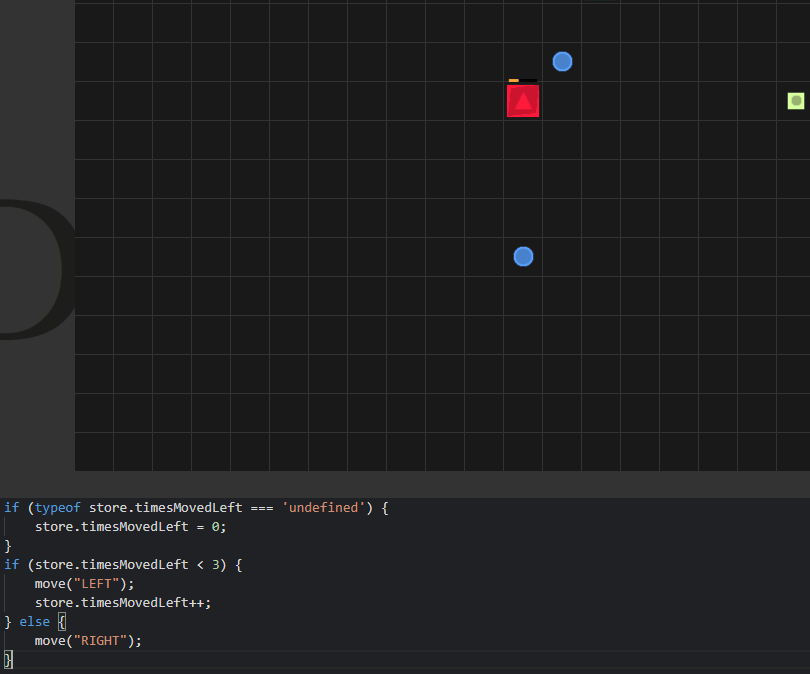
\includegraphics{game2.png}
	\caption{Design Code-Eingabe}
	\label{code-eingabe}
\end{figure}

\newpage

\section{Diskussion und Ausblick}
% Bespricht die erzielten ergebnisse bezüglich erwartbarkeit, aussagekraft, relevanz
% interpretation und validierung der resultate
% rückblick auf aufgabenstellung, erreicht oder nicht
% wie kann an die resultate angeschlossen werden (weitere forschungsarbeiten), welche chancen bieten die resultate
%

Projekt Darwin wurde gemäss unserer Planung erfolgreich umgesetzt. Wir haben alle Funktionen implementiert und können ein lauffähiges Spiel präsentieren.

\subsection{Workflow}

Die automatisierte Build-Pipeline hat sich als sehr wichtig herausgestellt, um während der Entwicklungsphase mit mehreren Entwicklern effizient arbeiten zu können. Der Workflow gewährleistet, dass ausschliesslich funktionierender Code deployed wird. Dies hat den Vorteil, dass nachfolgende Entwickler nicht blockiert werden, falls eingecheckter Code nicht kompiliert. Auch das Testing kann deshalb verzögerungsfrei starten, da es nicht auf eine nicht funktionierende Umgebung warten muss.

\subsection{Benutzeroberfläche}

Die einfach gehaltene Grafik und das schnörkellose Design unterstützen den Spieler dabei, sich auf das Wesentliche zu konzentrieren.
Die angebotene Hilfe mit Beispielen erweist sich als sehr nützlich, insbesondere für Programmier-Anfänger. Schliesslich soll man durch das Spiel auch lernen, zu programmieren.

\subsection{Spielfeld}

Die Grafik der Icons auf dem Spielfeld war zu Beginn etwas aufwendiger geplant, das Team wollte Figuren aus der ''Wilhelm Tell''-Sage benutzen. Wir haben uns jedoch früh dagegen entschieden, komplexe Icons zu entwerfen. Die aufwendige Darstellung hätte dem Spiel zwar ein interessantes Thema gegeben, jedoch durch den höheren Aufwand andere Funktionen des Spiels verzögert. Die jetzt verwendeten geometrischen Formen sind sehr klar, für den Spieler gut erkennbar und passen auch insgesamt gut zur Grafik. Wir sind deshalb mit dieser Anpassung zufrieden.

\subsection{Spielführung}

Die Regeln des Spiels sind sehr einfach gehalten, das hilft dem Spieler, sich auf das Hauptziel zu konzentrieren, nämlich das Programmieren zu erlernen und seine Strategie in Code umzusetzen.

\subsection{Scrum}
Scrum ermöglicht, den Entwicklungsprozess strukturiert und effizient zu gestalten. Ein agiles Umfeld wie Scrum hilft, die auftretenden Probleme besser und schneller zu bewältigen. Wir sind deshalb froh, dass wir dieses Framework benutzt haben.

\subsection{Ausblick}

Es gibt diverse Erweiterungsmöglichkeiten für das Spiel. Einige werden im Folgenden näher beschrieben:

\subsubsection{Benutzeroberfläche}
Es ist möglich, das ursprünglich angedachte, komplexere Icon-Set zu implementieren. Der Spieler könnte sich damit vielleicht besser mit der Geschichte identifizieren. Dies hat für den Product Owner allerdings im Moment keine Priorität, da der Aufwand für die Erstellung des Icon-Sets im Vergleich zum Nutzen zu gross ist.

\subsubsection{Befehlssatz}
In Zukunft können die zur Verfügung stehenden Befehle erweitert werden, zum Beispiel durch weiterführende Levels, sodass auch neue Strategien möglich werden. Damit könnte man zum Beispiel die Spieler durch verschiedene Lernstufen begleiten und sie können ihre Fähigkeiten Schritt für Schritt verbessern.

\subsubsection{Spielmodus}
Es ist auch möglich, verschiedene neue Spielobjekte mit einzuführen. Zum Beispiel solche, die man sammeln kann oder denen man ausweichen muss. Es besteht aber die Gefahr, dass das Spiel dadurch unnötig verkompliziert wird, ohne dass der Spieler seine Programmierfähigkeiten verbessert. Daher müssen diese Anpassungen sehr vorsichtig vorgenommen werden.

\newpage

% Literaturverzeichnis
%Beispiele Grundmuster Harvard-System:
%Deutsch:\\
%Name, Vorname (Jahreszahl): \textit{Titel. Unertitel.} ev. Vorname Name (Hrsg.), ev. Bd., ev. Auflage. Verlagsort: Verlag 
%Englisch:\\
%Author surname, Initials. (Year). title. ed. City: Publisher, p.Pages Used.

% Online-Publikation Grundmuster:
% Vorname-Initiale. Autorname. (Datum). titel (Ausgabe) [Online]. URL: url [Stand: Abfragedatum]

\begin{otherlanguage}{german}
\printbibliography
\end{otherlanguage}

\begin{otherlanguage}{german}
\listoffigures
\end{otherlanguage}
\end{document}
